
\subsection{Single particle responses and LCE estimation}

\begin{figure}[hbtp]
    \centering
    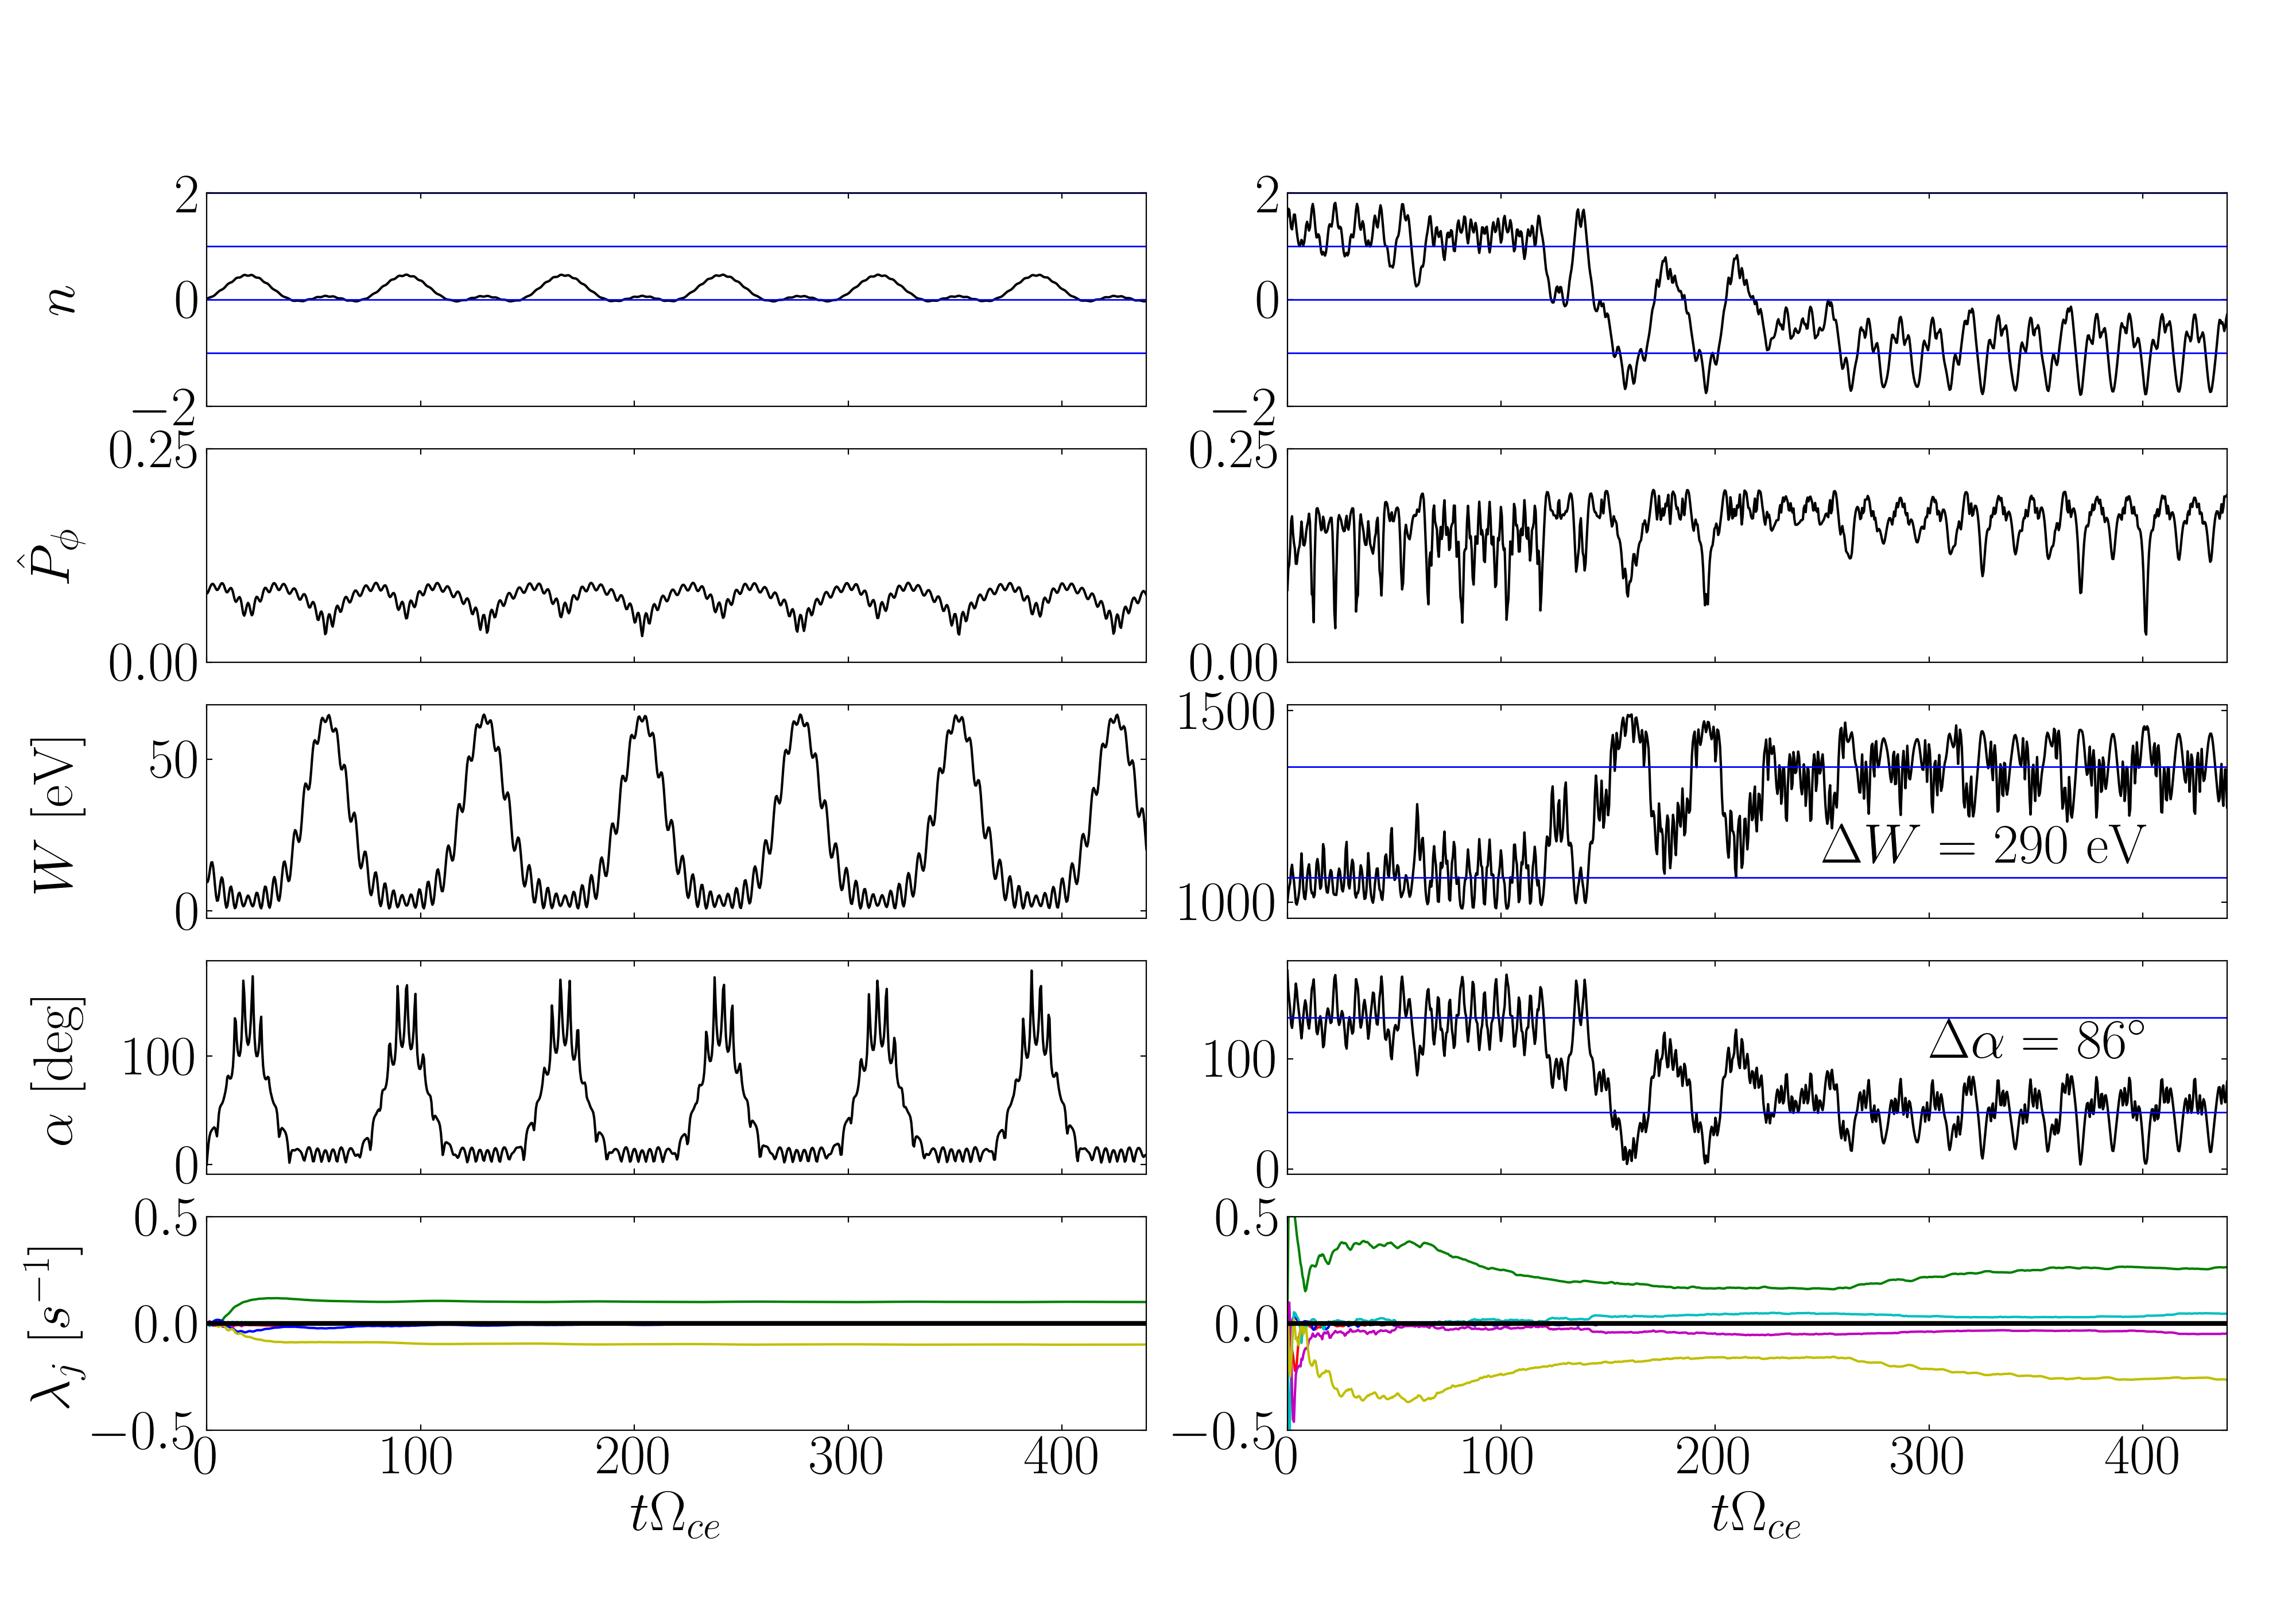
\includegraphics[width=\textwidth]{compare_time_series.png}
    \caption{Time series of two electrons with initial conditions
    $(W_0,\alpha_0)$ = (10\,\si{eV},0$^\circ$) (left column) and
    $(W_0,\alpha_0)$ = (1\,\si{keV},180$^\circ$) (right column) interacting with
a single 65$^\circ$ whistler at 1 AU. The first row shows the resonant mismatch
$n$ calculated from \cref{eq:resonant_condition}. The second row is the
adiabatic invariant $\hat{P_\phi}$ conjugate to the transformed gyrophase
$\phi$. The third row is the kinetic energy $W=(\gamma-1)mc^2$. The fourth row
is the pitch angle $\alpha=\cos^{-1}\qty(v_z/v)$. The last row shows the
Lyapunov exponent spectrum $\lambda_j$ in colors, each corresponds to one of
the six dimensions in the 6-ball, and the LCE in black.}
    \label{fig:compare_time_series}
\end{figure}

\cref{fig:compare_time_series} shows the dramatic differences in the response of
two particles. One is fast (1\,\si{keV}) and the other is fairly slow
(10\,\si{eV}).  For the slow particle, we can see quasi-periodic motion where it
enters the Landau resonance $(n=0)$ briefly, resulting in an energization in $W$
while the pitch angle $\alpha$ remains constant. Note that the adiabatic
invariant $\hat{P_\phi}=P_\phi-n\hat{P_\zeta}$ is modulated by $G_n\propto
\rho J_n'(k_\bot\rho)$ for small $P_\|$ and $\rho$ near the resonance. So for
the slow particle, the fluctuations in $\hat{P_\phi}$ are small ($\sim0.01$)
near $n=0$. For the 1\,\si{keV} particle, the energization and scattering is
much more significant. As it flips from $n=1$ (the fundamental cyclotron
resonance) to $n=-1$, the kinetic energy $W$ is increased by 30\% of its initial energy and it is scattered by $86^\circ$. It is also worth noticing that the particle sporadically enters and exits a resonance in a short time scale, leading to spikes of the order of $0.1$ in the adiabatic invariant.


From \cref{sec:particle_dynamics}, the particle's energy and
adiabatic invariant are not conserved when it crosses a resonance. So these
conservation laws are momentarily broken. However, in this non-relativistic
energy range ($W\sim1$\,\si{keV}), the resonance crossing occurs frequently and
sporadically, resulting in less distinctive changes than an example already
shown in \cref{fig:resonance_crossing}, which is typical of wave-particle interactions in the radiation belts. This is due to the small wave fields assumption in \cref{sec:particle_dynamics}. Specifically, it is required
that $\abs{qA/mu_{\max}}\ll 1$ for the radiation belts conditions to
apply. However, it is shown in
\cref{fig:potential_dominance}  that the initiated particles have maximum 
velocity $u_{\max}$ such that $\abs{qA/mu_{\max}}$ is $\sim\mathcal{O}(0.1)$. 
So the simulation of large amplitude whistler waves result in nonlinear effects 
much different from radiation belts context. For the sake of demonstration, a 
comparably similar behavior can be obtained by simulating relativistic 
electrons. \cref{fig:relativistic_resonance_crossing} shows the distinctive 
jumps in the resonant harmonic $n$ and the adiabatic invariant $\hat{P_\phi}$ 
for a 1\,\si{MeV} electron under the interaction of the same wave parameters as 
those in \cref{fig:compare_time_series}. Note that the trapping occurs both 
near a resonance and outside a resonance. A method to identify trapping
occurences has not yet been developed.

\begin{figure}[hbtp]
    \centering
    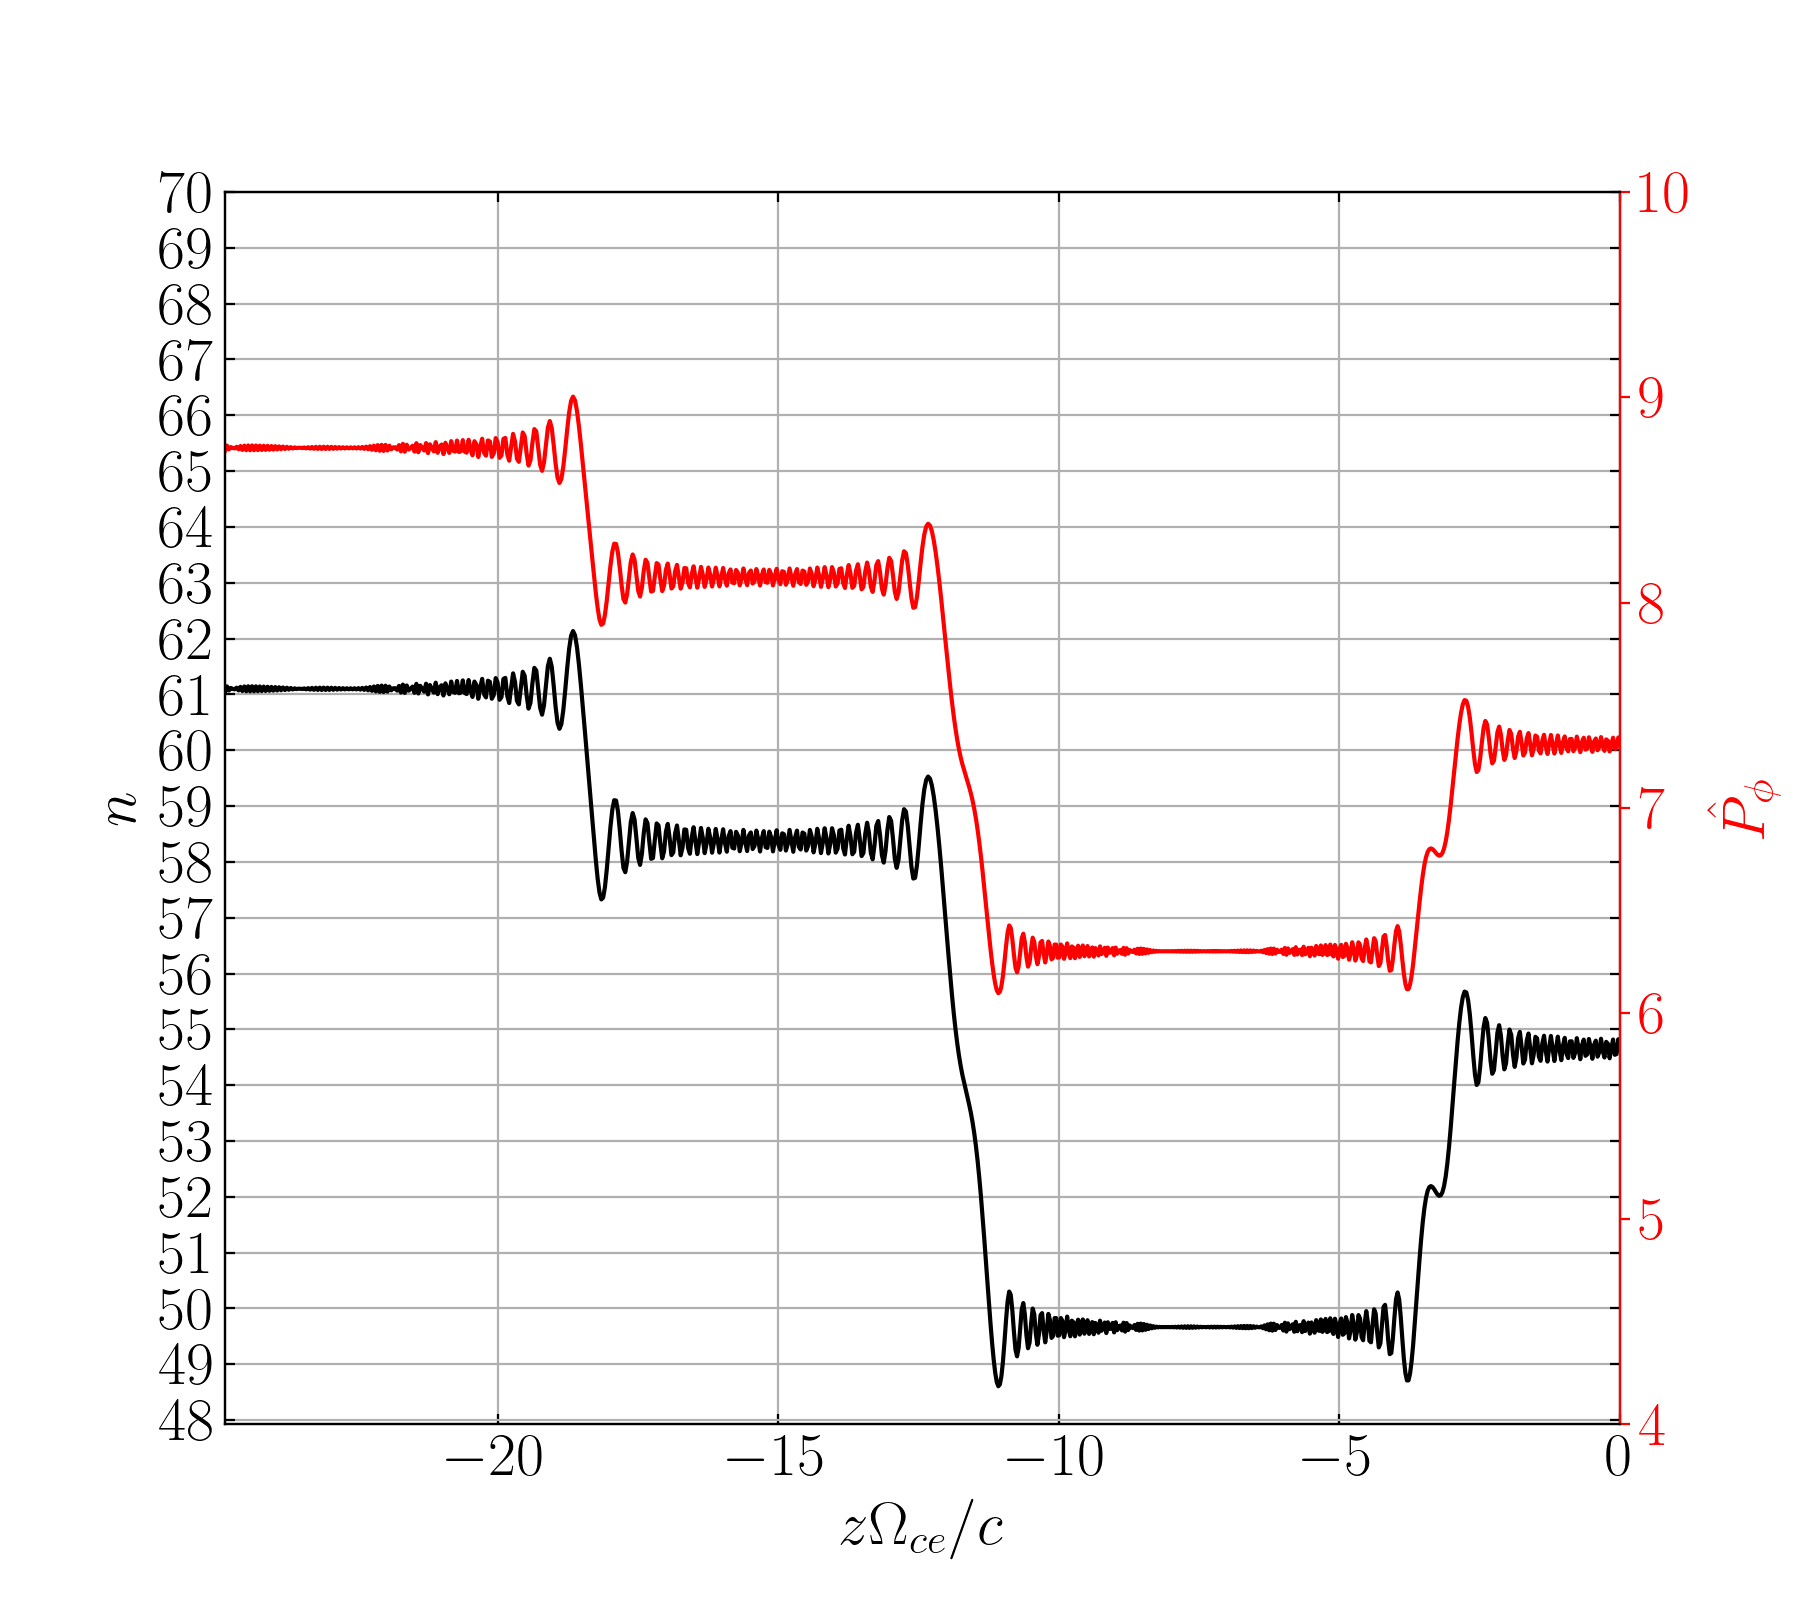
\includegraphics[width=0.7\textwidth]{diagnostics_resonance_crossing.png}
    \caption{Resonance crossing of a 1\,\si{MeV} particle interacting with a
    single 65$^\circ$ whistler at 1 AU. The left (black) axis plots the
resonance mismatch $n$, and the right (red) axis shows the adiabatic invariant
$\hat{P_\phi}$.}
    \label{fig:relativistic_resonance_crossing}
\end{figure}

The Lyapunov exponent spectrum, i.e., the different components $\lambda_j$, is
plotted in different colors in the last row of \cref{fig:compare_time_series}.
None of the components have any physical significance because the 6-D ball is free to rotate along the particle trajectory in our
calculations as described in \cref{sec:sim_LCE}. But they signify that there is
always at least one chaotic component, which corresponds to the sporadic
violation of the conservation of the adiabatic invariant inherent in our system.
Now, it is their sum, the LCE, that is important. As expected, the Lyapunov
exponents converge after a transient period at the beginning. So the estimation
of the LCE after a sufficiently long time period is constant. This enables the
estimation of the best step size to use without running very long simulations.
\cref{fig:LCE_compare} shows the LCE of all of the initiated particles after it
has reached convergence. The maximum LCE is $\lambda\sim10^{-3}$ in both cases.
Thus, for a step size of $\Delta t=10^{-4}$, the volume of the 6-D ball scales
as $\exp\qty(\lambda N\Delta t)\sim 1$ as long as the number of steps
$N\lesssim10^{7}$. In the physical parameters of interest, $10^7$ steps 
correspond to $\sim 60$ wave periods, which is a sufficiently long simulation 
time to study the responses.

\begin{figure}
    \centering
    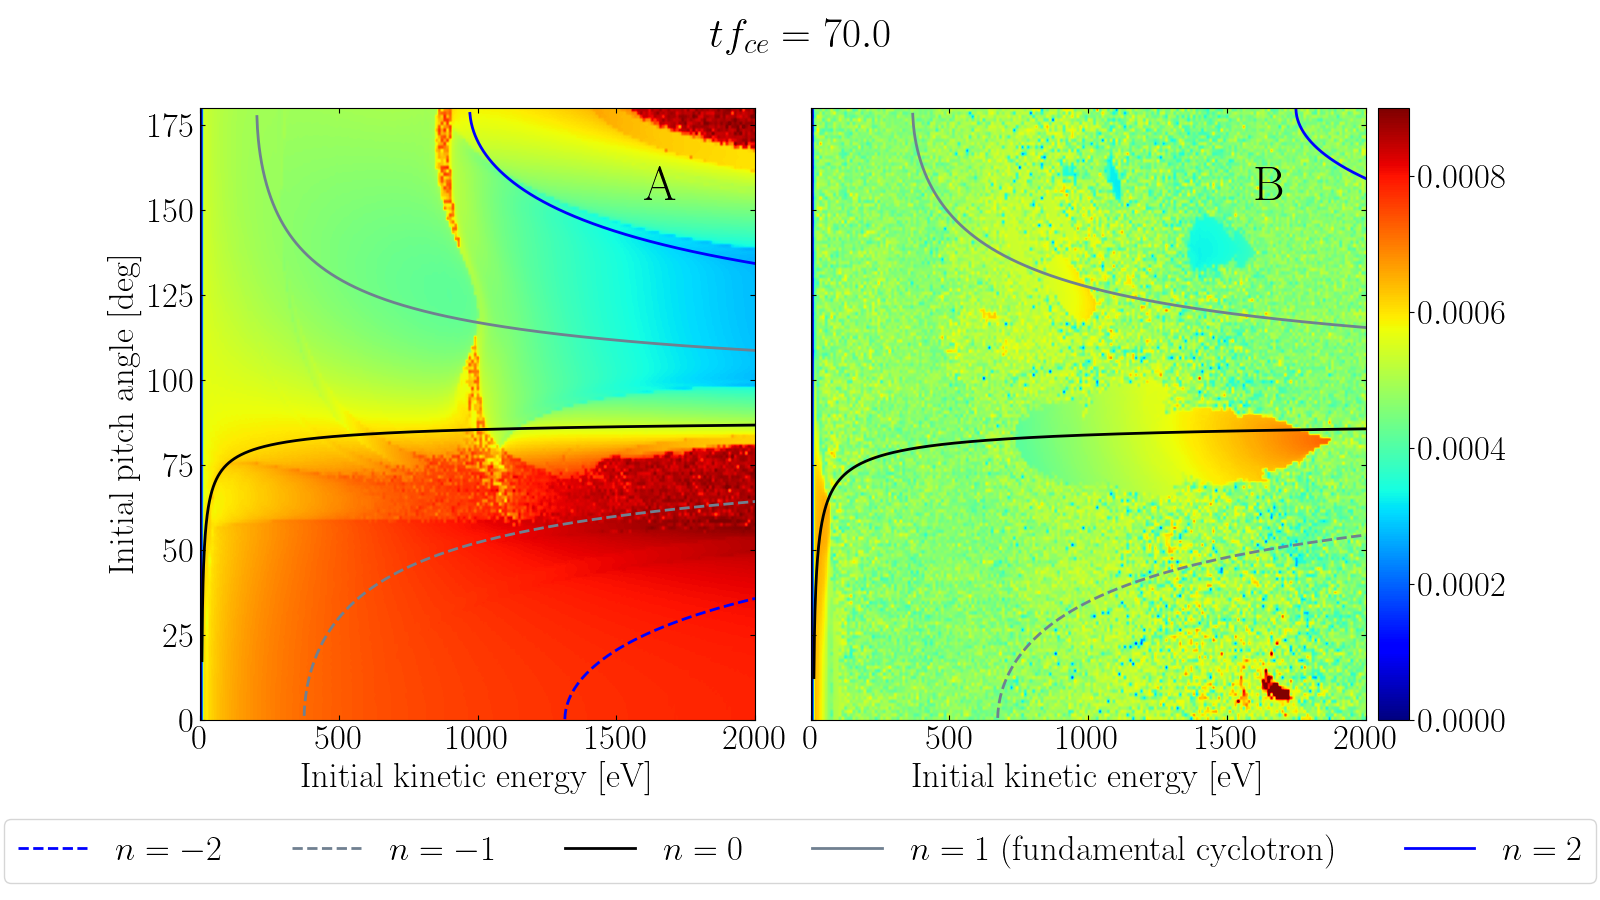
\includegraphics[width=\textwidth]{LCE_compare.png}
    \caption{The LCE of the simulations with a single $5^\circ$ whistler (A) and
    a single $65^\circ$ whistler (B) at 1 AU after a sufficient simulation
period for its convergence.}
\label{fig:LCE_compare}
\end{figure}
